\documentclass[
  unicode,a4paper,9pt,
  % aspectratio=169,
  xcolor = {dvipsnames,svgnames},
  hyperref ={colorlinks=true,citecolor=Navy,linkcolor=NavyBlue,urlcolor=purple},
  ja=standard,lualatex
]{beamer}
\renewcommand{\baselinestretch}{1.4}

% ---fonts---
\PassOptionsToPackage{quiet}{fontspec}
\usefonttheme{serif}
\mathversion{bold}
\usepackage{luatexja-fontspec}
\setmainfont{TeX Gyre Termes}
\setmainjfont{Noto Sans CJK JP}
% \setmainjfont[BoldFont = HaranoAjiGothic-Regular]{HaranoAjiMincho}
% \setmainjfont[BoldFont = IPAGothic]{IPAMincho}
\setmathrm{Latin Modern Roman}
% \usepackage{newtxmath}

\usepackage{newunicodechar}
\newunicodechar{–}{-}

% ---refer `texdoc xcolor' at the command line---

% ---Display \subsubsection at the Index
% \setcounter{tocdepth}{3}

% ---Setting about the geometry of the document----
% \usepackage{a4wide}
% \pagestyle{empty}

% ---Physics and Math Packages---
\usepackage{amssymb,amsfonts,amsthm,mathtools}
\usepackage{physics,braket,bm,slashed}

% ---underline---
\usepackage[normalem]{ulem}

% ---cancel---
\usepackage{cancel}

% --- surround the texts or equations
\usepackage{fancybox,ascmac}

% ---settings of theorem environment---
\usepackage{amsthm}
\theoremstyle{definition}

% ---settings of proof environment---
\renewcommand{\proofname}{\textbf{証明}}
\renewcommand{\qedsymbol}{$\blacksquare$}

% ---Insert the figure (If insert the `draft' at the option, the process becomes faster.)---
\usepackage{graphicx}
% \usepackage{subcaption}

% ----Add a link to a text---
\usepackage{url,hyperref}
\usepackage{xcolor}

% ---Tikz---
\usepackage{tikz,pgf,pgfplots,circuitikz}
\pgfplotsset{compat=1.15}
\usetikzlibrary{intersections,arrows.meta,angles,calc,3d,decorations.pathmorphing,positioning}

% ---Add the section number to the equation, figure, and table number---
\makeatletter
   \renewcommand{\theequation}{\thesection.\arabic{equation}}
   \@addtoreset{equation}{section}
   
   \renewcommand{\thefigure}{\thesection.\arabic{figure}}
   \@addtoreset{figure}{section}
   
   \renewcommand{\thetable}{\thesection.\arabic{table}}
   \@addtoreset{table}{section}
\makeatother

% ---enumerate---
% \renewcommand{\labelenumi}{$\arabic{enumi}.$}
% \renewcommand{\labelenumii}{$(\arabic{enumii})$}

% ---beamer settings---
\usefonttheme{professionalfonts}
\usecolortheme{seahorse}
\setbeamercolor{structure}{fg=white}
\setbeamercolor{local structure}{fg=red}
\setbeamertemplate{itemize item}[ball]
\setbeamertemplate{enumerate item}[circle]
\setbeamercolor{bibliography entry author}{fg=black}
\setbeamercolor{bibliography item}{fg=black}
\setbeamercolor{alerted text}{fg=RoyalBlue}
\setbeamertemplate{frametitle continuation}{}
\setbeamertemplate{footline}[frame number]
\setbeamertemplate{navigation symbols}{} 
\setbeamersize{text margin left=10pt, text margin right=10pt}

% ---tcolorbox---
\usepackage{tcolorbox}
\tcbuselibrary{theorems}
\tcbuselibrary{raster}
\tcbuselibrary{skins}
\newtcolorbox{bluebox}[2][]{enhanced,
colframe=RoyalBlue!40!white,
colback=RoyalBlue!10!white,
coltitle=black,
drop fuzzy shadow, title={#2}
,#1}
\newtcolorbox{redbox}[2][]{enhanced,
colframe=DarkRed!40!white,
colback=DarkRed!10!white,
coltitle=black,
drop fuzzy shadow, title={#2}
,#1}

% ---tcolorbox---
\usepackage{tcolorbox}
\tcbuselibrary{raster,skins,breakable}
\newtcolorbox{graybox}[1][]{frame empty, colback=black!10!white, sharp corners}

% ---Ignore the Warnings---
\usepackage{silence}
\WarningFilter{latexfont}{Some font shapes}
\WarningFilter{latexfont}{Font shape}
\WarningFilter{latexfont}{Size substitutions}
\ExplSyntaxOn
\msg_redirect_name:nnn{hooks}{generic-deprecated}{none}
\ExplSyntaxOff

% ---Citation on the slides---
\newcommand*{\citefone}[2]{
  \begin{tikzpicture}[remember picture, overlay]
    \node[anchor=north east, align=left] at ($(current page.north east)-(0,0.0)$){
    {\tiny
      \cite{#1}
      #2
    }
    };
  \end{tikzpicture}

  \vspace*{-20pt}
}

\newcommand*{\citeftwo}[4]{
  \begin{tikzpicture}[remember picture, overlay]
    \node[anchor=north east, align=left] at ($(current page.north east)-(0,0.0)$){
    {\tiny
      \cite{#1}
      #2
    }
    \\[-2.4ex]
    {\tiny
      \cite{#3}
      #4
    }
    };
  \end{tikzpicture}

  \vspace*{-20pt}
}

\newcommand*{\citefthree}[6]{
  \begin{tikzpicture}[remember picture, overlay]
    \node[anchor=north east, align=left] at ($(current page.north east)-(0,0.0)$){
    {\tiny
      \cite{#1}
      #2
    }
    \\[-2.4ex]
    {\tiny
      \cite{#3}
      #4
    }
    \\[-2.4ex]
    {\tiny
      \cite{#5}
      #6
    }
    };
  \end{tikzpicture}

  \vspace*{-20pt}
}

\newcommand*{\citefonev}[3]{
  \begin{tikzpicture}[remember picture, overlay]
    \node[anchor=north east, align=left, text width=#3cm] at ($(current page.north east)-(0,0.0)$){
    {{\fontsize{5pt}{0pt}\selectfont
      \cite{#1}
      #2\par}
    }
    };
  \end{tikzpicture}

  \vspace*{-20pt}
}

\newcommand*{\citeftwov}[5]{
  \begin{tikzpicture}[remember picture, overlay]
    \node[anchor=north east, align=left, text width=#5cm] at ($(current page.north east)-(0,0.0)$){
    {{\fontsize{5pt}{0pt}\selectfont
      \cite{#1}
      #2\par}

      {\fontsize{5pt}{0pt}\selectfont
      \cite{#3}
      #4\par}
    }
    };
  \end{tikzpicture}

  \vspace*{-20pt}
}

\newcommand*{\citefthreev}[7]{
  \begin{tikzpicture}[remember picture, overlay]
    \node[anchor=north east, align=left, text width=#7cm] at ($(current page.north east)-(0,0.0)$){
    {{\fontsize{5pt}{0pt}\selectfont
    \cite{#1}
    #2\par}

    {\fontsize{5pt}{0pt}\selectfont
    \cite{#3}
    #4\par}

    {\fontsize{5pt}{0pt}\selectfont
    \cite{#5}
    #6\par}
    }
    };
  \end{tikzpicture}

  \vspace*{-20pt}
}


% ---Title---
\title{
  title
}
\author{
  author
}
\date{Last modified: \today}

\begin{document}

\nocite{Arkani-Hamed:2001uol}

\begin{frame}

  \setbeamertemplate{blocks}[rounded][shadow=true]
  \setbeamercolor{block body}{bg=LimeGreen!10!white, fg=black}
  \begin{block}{}
    \vspace*{5pt}

    \centering\Large
    Anomalies on orbifolds
    \\
    \normalsize
    Nima Arkani-Hamed, Andrew G. Cohen, Howard Georgi.
    \\
    \small
    \href{https://doi.org/10.1016/S0370-2693(01)00946-7}{Physics Letters B 516 (2001) 395–402},
    \href{https://doi.org/10.48550/arXiv.hep-th/0103135}{arxiv:hep-th/0103135}.

    \vspace*{5pt}
  \end{block}

  \begin{center}
    安倍研 M1 宮根一樹\\
    2024 5/7 (火)
  \end{center}

\end{frame}


\begin{frame}

  読んだ動機を話そうと思ったのですが、\pause
  \begin{center}
    「お前の読んだ理由なんてみんな1ミリも興味ない」
  \end{center}
  と言われてしまったので、(本当にそうなんだと思いますし)自粛します。

  \vspace*{10pt}

  以下の論文を紹介します\cite{Arkani-Hamed:2001uol}。
  \begin{figure}[ht]
    \centering
    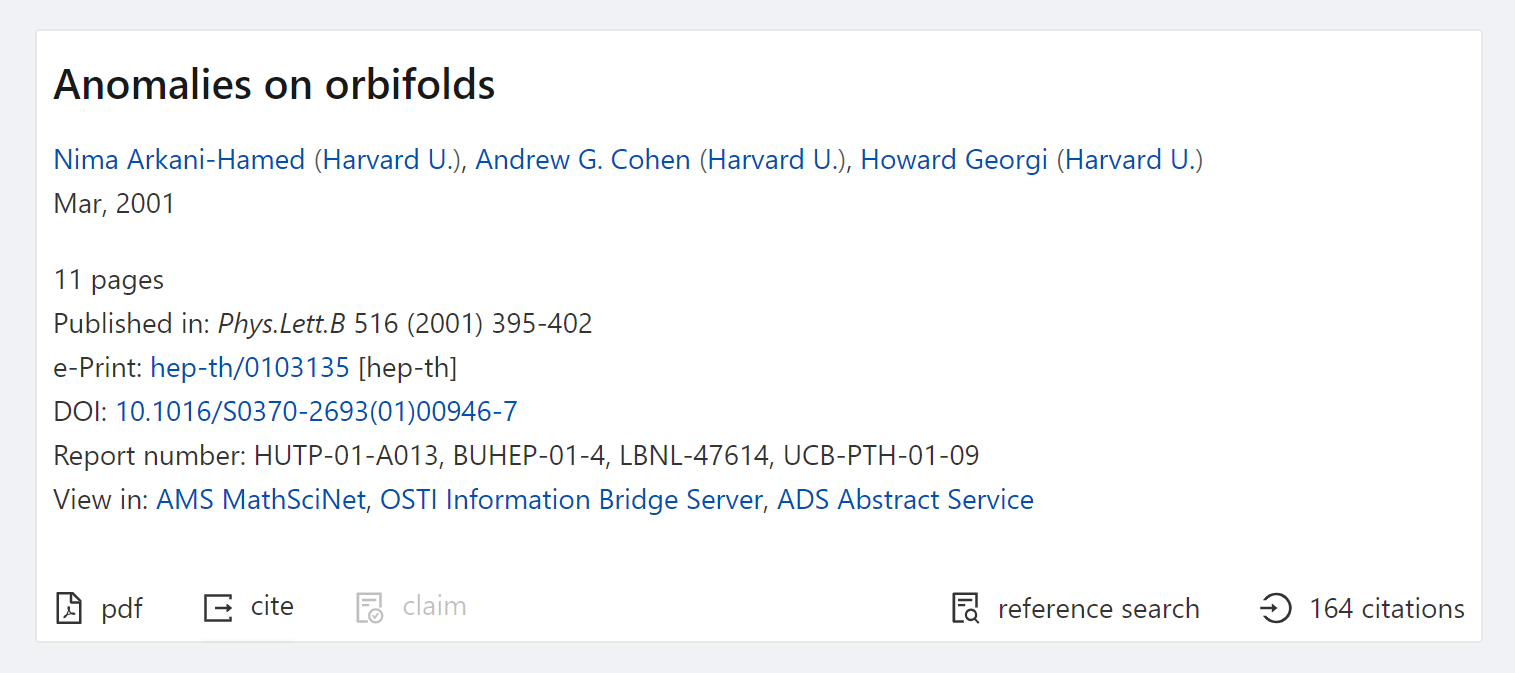
\includegraphics[width=0.7\textwidth]{fig/Arkani-Hamed2001uol.png}
  \end{figure}

  \citefone{Arkani-Hamed:2001uol}{N. Arkani-Hamed, A. G. Cohen, and H. Georgi, Physics Letters B 516 (2001) 395-402, arxiv:hep-th/0103135.}

\end{frame}


\section{イントロダクション}

\begin{frame}[plain]
  \huge \secname
\end{frame}

\subsection{アノマリー}

\begin{frame}{\subsecname}

  4次元の場合のカイラルアノマリーを確認する。

  \pause
  \vspace*{10pt}

  ゲージ場$A_{\mu}$と結合しているフェルミオン$\psi$を考える
  \begin{equation}
    \mathcal{L}
    =
    \bar{\psi}(i\slashed{\partial}-m)\psi
    +
    e\bar{\psi}\gamma^{\mu}\psi A_{\mu}
    \nonumber
  \end{equation}

  \vspace*{10pt}

  カイラル変換$\psi\rightarrow e^{i\gamma^{5}\alpha(x)}\psi$に対するネーターカレントの方程式は
  \begin{equation}
    \partial_{\mu}j^{\mu}_{5}
    =
    2im\bar{\psi}\gamma^{5}\psi
    ,\quad
    j^{\mu}_{5}
    =
    \bar{\psi}\gamma^{\mu}\gamma^{5}\psi
    \nonumber
  \end{equation}

\end{frame}



\begin{frame}

  \citeftwo{Peskin:1995}{M. E. Peskin and D. V. Schroeder, An Introduction to Quantum Field Theory. Addison-Wesley Pub. Co, Reading, Mass, 1995.}{Fujikawa:2001a}{藤川和男, ゲージ場の理論. 岩波書店, 2001.}

  しかし、これは古典論の結果

  \begin{equation}
    \partial_{\mu}
    (\bar{\psi}\gamma^{\mu}\gamma^{5}\psi)
    =
    2im\bar{\psi}\gamma^{5}\psi
    \nonumber
  \end{equation}

  摂動論でこの関係をチェックするには、ファインマンルールにしたがって以下のダイアグラムを計算してみればよい\cite{Peskin:1995,Fujikawa:2001a}。

  \begin{center}
    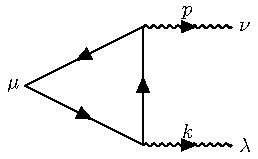
\includegraphics[width=0.4\textwidth]{fig/feynman_diag.pdf}    
  \end{center}

\end{frame}


\begin{frame}  

  \citefone{Fujikawa:2001b}{藤川和男, 経路積分と対称性の量子的破れ. 岩波書店, 東京, 2001.}

  前に示したダイアグラムを計算すると
  \begin{equation}
    \partial_{\mu}
    \ev*{\bar{\psi}\gamma^{\mu}\gamma^{5}\psi}
    =
    2im\ev*{\bar{\psi}\gamma^{5}\psi}
    +
    \textcolor{DarkGreen}{
      Q
    }
    ,\quad    
    \textcolor{DarkGreen}{
      Q
    }
    =
    \textcolor{DarkGreen}{
      \frac{e^2}{16\pi^2}\varepsilon^{\mu\nu\rho\sigma}\ev*{F_{\mu\nu}F_{\rho\sigma}}
    }
    \nonumber
  \end{equation}
  
  この余分な$\textcolor{DarkGreen}{Q}$は、ゲージ不変性を保って発散を正則化するときに生じる項

  \begin{center}
    この$\textcolor{DarkGreen}{Q}$を\textcolor{DarkRed}{カイラルアノマリー}という。    
  \end{center}  

  理論にアノマリーがあると、通常の量子論の定式化ができなくなることが知られている\cite{Fujikawa:2001b}。  

  よって、
  \setbeamertemplate{blocks}[rounded][shadow=true]
  \setbeamercolor{block body}{bg=Goldenrod!10!white, fg=black}
  \begin{block}{}
    \centering
    アノマリーが相殺されるように理論を作りたい
  \end{block}  

\end{frame}




\subsection{Kaluza-Klein理論とアノマリー}

\begin{frame}{\subsecname}

  高次元の時空を考え、余剰空間に周期条件を与えること(コンパクト化)によって、4次元有効理論を作る方法があり、それをKaluza-Klein理論という。

  \vspace*{5pt}

  特に、今回は5次元の時空$x^{M}=(x^{0},x^{1},\cdots,x^{4})$を考え、$x^{4}$の方向に$x^{4}\sim x^{4}+2L$の周期境界条件を課してコンパクト化する。

  \pause
  \vspace*{10pt}

  \setbeamertemplate{blocks}[rounded][shadow=true]
  \setbeamercolor{block body}{bg=RoyalBlue!10!white, fg=black}
  \begin{block}{}
    \centering
    \textcolor{Green}{5次元の理論}でのアノマリー相殺
    \\
    と
    \\
    \textcolor{FireBrick}{4次元有効理論}でのアノマリー相殺
    \\
    の対応
  \end{block}
  を調べたい。

\end{frame}


\begin{frame}

  一方で、カイラルアノマリーについては次のことが分かっている:

  \begin{itemize}
    \item 
    奇数次元の理論はクリフォード代数の性質から非カイラル\\
    $\hspace*{1cm}\ \longrightarrow\ $カイラルアノマリーは必ず相殺される
    \item 
    非カイラルな理論を$S^{1}$コンパクト化しても、4次元有効理論は非カイラル
  \end{itemize}

  \pause

  よって、5次元の理論をコンパクト化するだけでは、4次元のカイラルアノマリーが消えているのは明らか。\\

  そこで・・・  

\end{frame}

\subsection{オービフォールド\texorpdfstring{$S^{1}/Z_{2}$}{S1/Z2}}

\begin{frame}{オービフォールド$S^{1}/Z_{2}$}

  \citefonev{Choi:2020dws}{K.-S. Choi and C.-ŭ. Kim, Quarks and Leptons from Orbifolded Superstring, no. volume 954 in Lecture Notes in Physics. Springer, Cham, second edition ed., 2020.}{7}

  今回は、さらに\textcolor{Goldenrod}{オービフォールド}という境界条件を余剰空間に課す。
  
  \pause
  \vspace*{10pt}

  例えば、スカラー場の理論を考える
  \begin{equation}
    S
    =
    \int\dd^5 x\ 
    \left(  
      \frac{1}{2}\partial^{M}\Phi\partial_{M}\Phi
      -
      \frac{1}{2}m(x^{4})^2\Phi^2
    \right)
    \nonumber
  \end{equation}

  この理論に、$\Phi(x,x^{4})=\Phi(x,x^{4}+2L)$という境界条件に加えて
  \begin{equation}
    \Phi(x,x^{4})
    =
    \eta
    \Phi(x,-x^{4})
    \ ,\ 
    \eta=\pm 1
    \nonumber
  \end{equation}
  という境界条件を課す。  

\end{frame}

\begin{frame}

  \citefonev{Choi:2020dws}{K.-S. Choi and C.-ŭ. Kim, Quarks and Leptons from Orbifolded Superstring, no. volume 954 in Lecture Notes in Physics. Springer, Cham, second edition ed., 2020.}{7}

  まずは、周期境界条件$\Phi(x,x^{4})=\Phi(x,x^{4}+2L)$から
  \begin{equation}
    \Phi(x,x^{4})
    =
    \sum_{n=-\infty}^{\infty}\phi_{n}(x) \exp \left[ i\frac{n\pi}{L}x^{4} \right]
    \nonumber
  \end{equation}
  とフーリエ展開できる。

  \vspace*{5pt}

  さらに、オービフォールドの境界条件$\Phi(x,x^{4})=-\Phi(x,-x^{4})$を課すと$\phi_{n}(x)+\phi_{-n}(x)=0$という条件になる

  \vspace*{5pt}

  この条件により、$n=0$のモード$\phi_{0}(x)$は消えることがわかる

  \pause
  \vspace*{5pt}

  \setbeamertemplate{blocks}[rounded][shadow=true]
  \setbeamercolor{block body}{bg=RoyalBlue!10!white, fg=black}
  \begin{block}{}
    \centering
    境界条件をうまく選べば、ゼロモードの場を消したり残したりできるため
    \\
    4次元の有効理論を作るときに嬉しい
  \end{block}
  ので、調べられている。

\end{frame}


\subsection{本論文の流れ・まとめ}

\begin{frame}
  \frametitle{\subsecname}

  同様のことが$x^{4}=L$の点でも起こることがわかる

  \vspace*{5pt}

  $x=0,L$の点(固定点)では、ゼロモードがカイラルになる

  $\qquad\rightarrow\ $アノマリーが5次元の理論でも現れる可能性がある

  $\qquad\rightarrow\ $4次元有効理論でのアノマリーとの関係は?

  \pause
  \vspace*{5pt}

  \uline{議論の流れ}

  \begin{itemize}
    \item 
    余剰空間方向の場の境界条件を設定、モード展開
    \item 
    それを元のラグランジアンに代入$\rightarrow$カレントを計算
    \item 
    有効理論のアノマリーと元の理論のアノマリーの関係の議論
  \end{itemize}

  \vspace*{5pt}

  今回、得られる結果は
  \begin{equation*}
    \partial_{C}j^{C}
    =
    \frac{1}{2}\left[ \delta(x)+\delta(x-L) \right]Q
    \quad
    (C=0,1,2,3,4)
  \end{equation*}

  \setbeamertemplate{blocks}[rounded][shadow=true]
  \setbeamercolor{block body}{bg=Green!10!white, fg=black}
  \begin{block}{}
    \centering
    5次元のカレントの保存も量子補正によって破れることがある。
  \end{block}

\end{frame}


\section{本論}

\begin{frame}[plain]
  \huge \secname
\end{frame}

\subsection{4次元のアノマリー}

\begin{frame}
  \frametitle{\subsecname} 

  最初のレビューの部分で良く分からない記述がありました。

  \begin{center}
    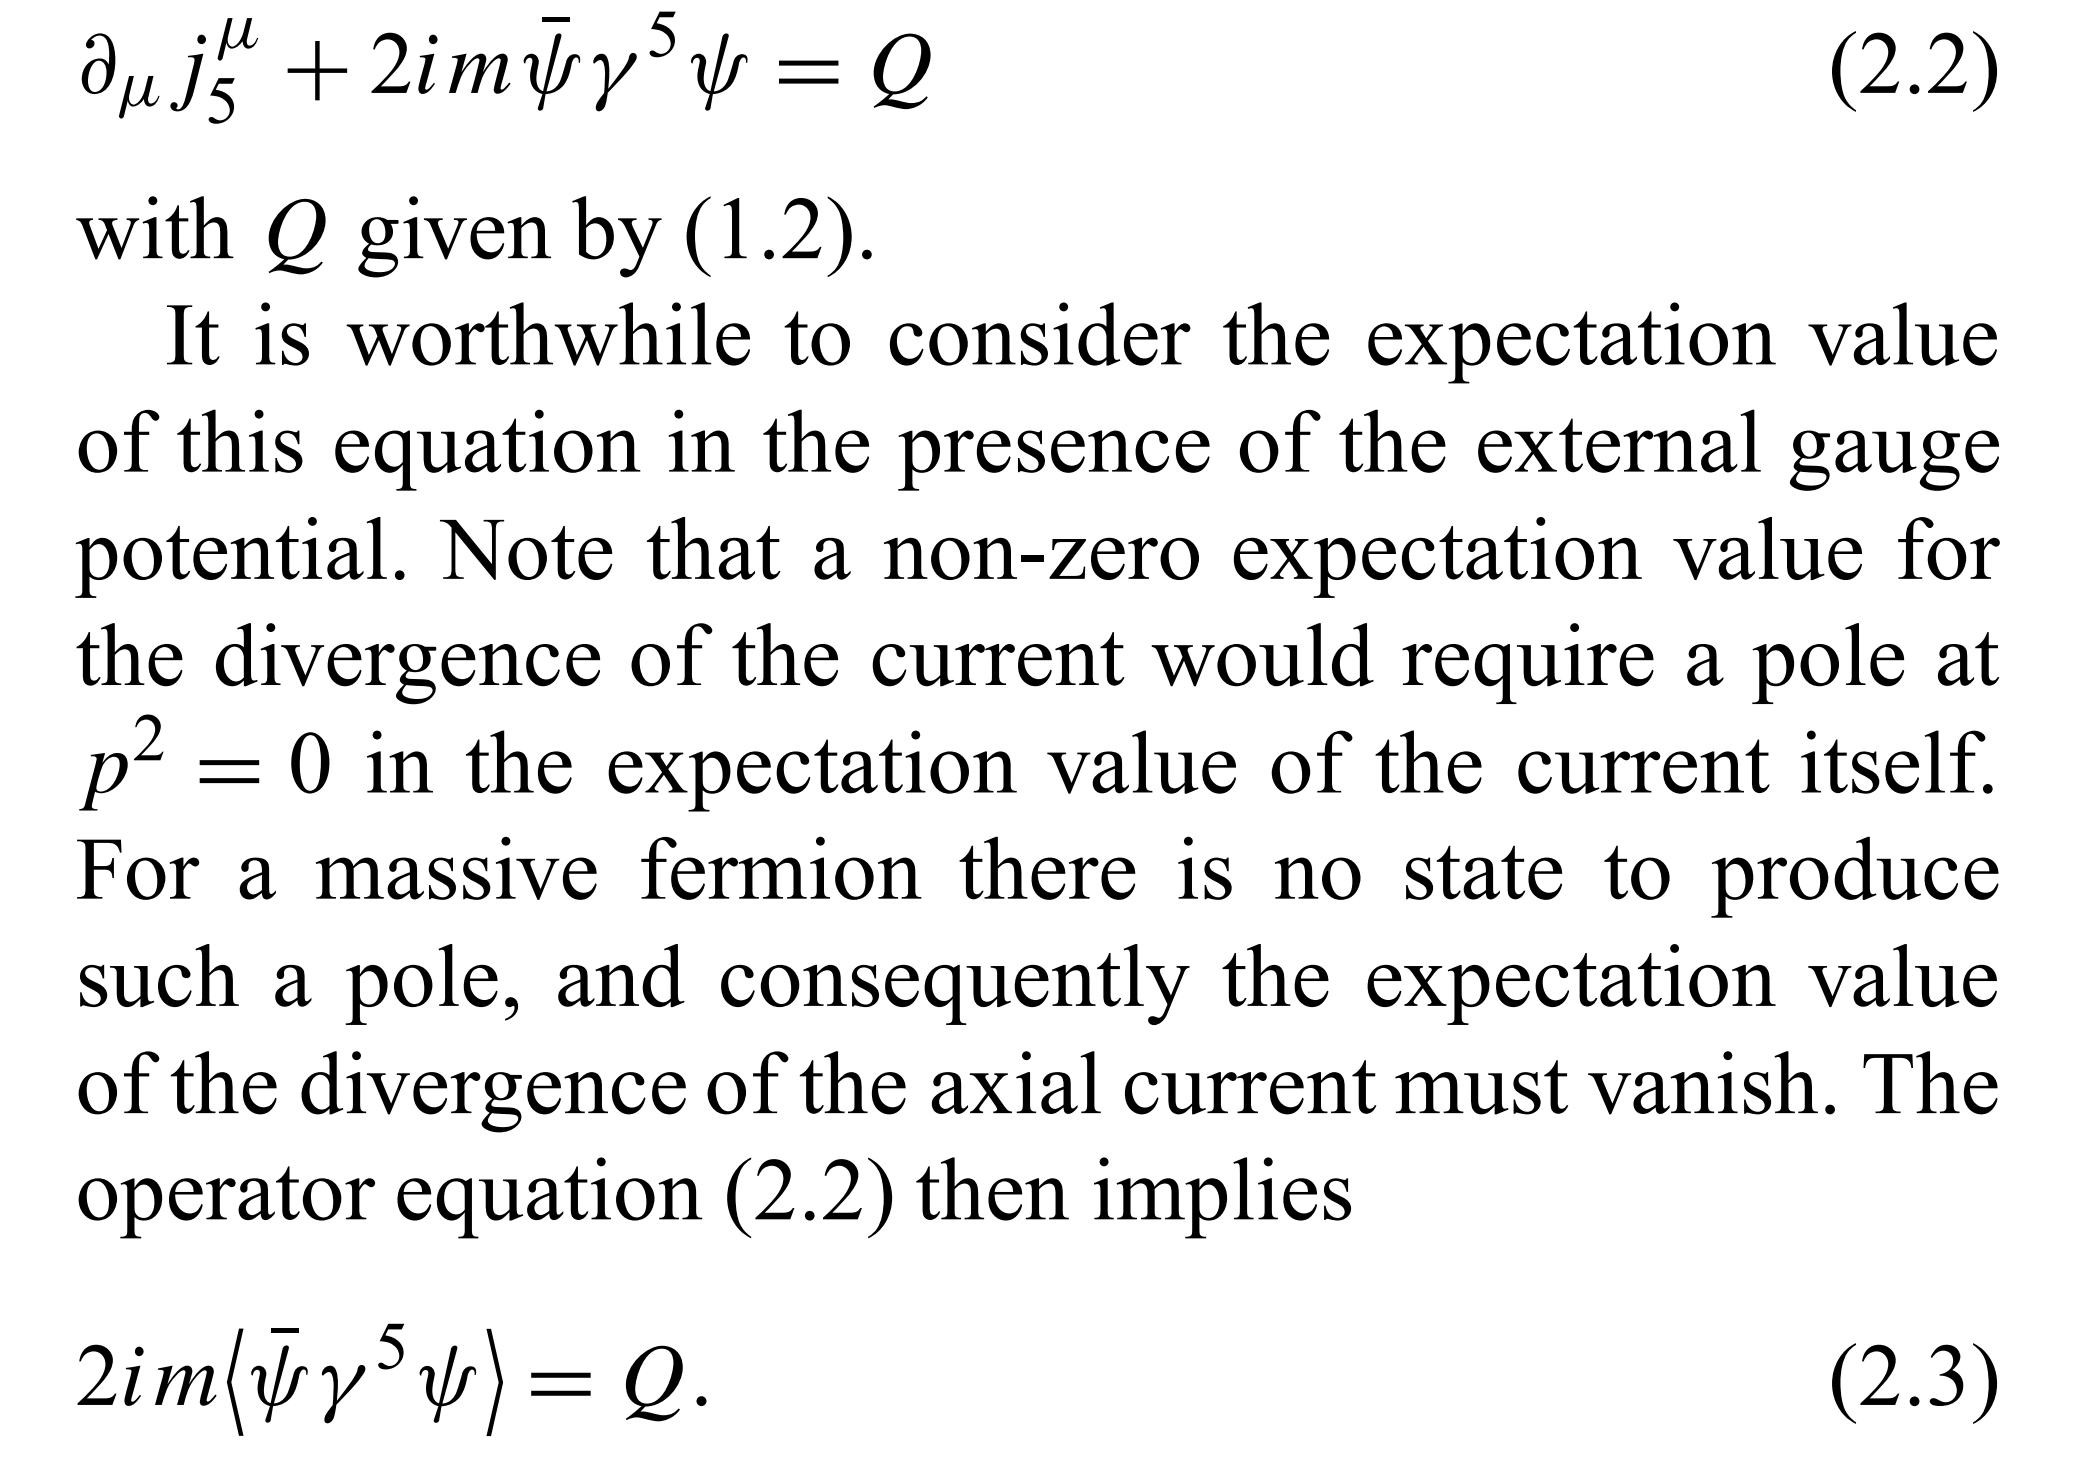
\includegraphics[width=0.8\textwidth]{fig/text_01.png}    
  \end{center}

\end{frame}

\begin{frame}

  \citefonev{Coleman:1982yg}{S. Coleman and B. Grossman, Nuclear Physics B 203 (1982) 205-220.}{6}

  おそらく
  \begin{center}
    「massiveなら極は$p^2=0$のところにないので、$\ev*{\partial_{\mu}j^{\mu}_{5}}=0$」
  \end{center}
  ということ?

  \vspace*{5pt}

  複数の場$\psi_{i}, A_{ij}^{\mu}$とチャージ$q_{i}$がある場合は
  \begin{equation*}
    \partial_{\mu}j^{\mu}_{5}
    +
    2i\bar{\psi}M\gamma^{5}\psi
    =
    \frac{1}{2}Q
    ,\ 
    Q
    =
    \frac{1}{16\pi^2}
    \tr qF\tilde{F}
  \end{equation*}
  となる。

  \vspace*{5pt}

  先行研究\cite{Coleman:1982yg}によると、無質量モードのみが真空期待値の計算に寄与してきて
  \begin{equation*}
    \ev*{\partial_{\mu}j^{\mu}_{5}}
    =
    \frac{1}{32\pi^2}
    \tr
    \left[  
      P_{0}qP_{0}FP_{0}\tilde{F}
    \right] 
    \label{eqn:massless_anomaly}
  \end{equation*}  
  $P_{0}$は無質量モードへの射影。

\end{frame}

\subsection{セットアップ}

\begin{frame}
  \frametitle{\subsecname}

  時空は5次元$x^{C}=(x^{\mu},x_{4})$

  \uline{作用}
  \begin{gather}
    S
    =
    \int\dd^4 x
    \int_{0}^{L}\dd x_{4}\ 
    \bar{\psi}(i\slashed{D}-\textcolor{DarkRed}{\gamma_{4}D_{4}}-m(x_{4}))\psi
    \nonumber
    \\
    \slashed{D}
    \equiv
    \gamma^{\mu}D_{\mu}
    ,\ 
    D_{C}
    =
    \partial_{C}-iA_{C}
    ,\ 
    \gamma_{4}
    \equiv
    -i\gamma^{5}
    \nonumber
  \end{gather}


  \uline{境界条件}:  周期境界条件$x_{4}\sim x_{4}+2L$とオービフォールド
  \begin{gather}
    \psi(x,x_{4})
    =
    \gamma^{5}\psi(x,-x_{4})
    \nonumber
    \\
    A_{\mu}(x,x_{4})
    =
    A_{\mu}(x,-x_{4})
    \nonumber
    \\
    A_{4}(x,x_{4})
    =
    -A_{4}(x,-x_{4})
    \nonumber
    \\
    \Rightarrow
    \quad
    m(x_4)
    =
    m(2L+x_4)
    =
    -m(-x_{4})
    \nonumber
  \end{gather}

\end{frame}

\begin{frame}

  また、$\psi(x,x_{4})$をカイラリティーで分類
  \begin{equation}
    \psi
    =
    \psi_{+}
    +
    \psi_{-}
    ,\ 
    \gamma^{5}\psi_{\pm}
    =
    \pm\psi_{\pm}
    \nonumber
  \end{equation}

  \vspace*{5pt}

  \uline{ゲージ変換}: ローカルな$U(1)$

  \begin{gather}
    \psi(x,x_{4})
    \rightarrow
    e^{i\phi(x,x_{4})}
    \psi(x,x_{4})
    \nonumber
    \\
    A_{C}(x,x_{4})
    \rightarrow
    A_{C}(x,x_{4})
    -
    i\partial_{C}\phi(x,x_{4})
    \nonumber
    \\
    \Rightarrow\quad
    \phi(x,x_{4})
    =
    \phi(x,x_{4}+2L)
    =
    \phi(x,-x_{4})
    \nonumber
  \end{gather}

\end{frame}


\subsection{アノマリーの計算}

\begin{frame}
  \frametitle{\subsecname}

  以下、$A_{4}=0$とゲージ固定する。

  \vspace*{5pt}

  KKモード展開は次の通り
  \begin{equation}
    \psi_{\pm}(x,x_{4})
    =
    \sum_{M}
    \psi_{M\pm}(x)\xi^{\pm}_{M}(x_{4})
    \nonumber
  \end{equation}

  ただし、
  \begin{align}
    \left[\vphantom{\frac{1}{2}}
      -\textcolor{DarkGreen}{i}\partial_{4}+m(x_{4})
    \right]
    \xi_{M}^{+}(x_{4})
    =
    M\xi_{M}^{+}
    \quad
    (M\geq0)
    \nonumber
    \\
    \left[\vphantom{\frac{1}{2}}
      \textcolor{DarkGreen}{i}\partial_{4}+m(x_{4})
    \right]
    \xi_{M}^{-}(x_{4})
    =
    M\xi_{M}^{-}(x_{4})
    \quad
    (\textcolor{DarkRed}{M>0})
    \nonumber
  \end{align}

  ($\textcolor{DarkGreen}{i}$忘れはおそらくタイポ?)

  このモード展開の基底は完全性を満たす。内積は積分。
  \begin{equation*}
    \sum_{M}\xi^{\pm}_{M}(x)\xi^{\pm}_{M}(y)
    =
    \delta(x-y)
  \end{equation*}

\end{frame}

\begin{frame}  

  KKモード展開
  \begin{equation}
    \psi_{\pm}(x,x_{4})
    =
    \sum_{M}
    \psi_{M\pm}(x)\xi^{\pm}_{M}(x_{4})
    \nonumber
  \end{equation}
  \begin{itemize}
    \item 
    元の作用に代入
    \item 
    $x_{4}$の方向を$0$から$L$で積分
  \end{itemize}
  すると
  \begin{align}
    S
    &=
    \int\dd^4 x\ 
    \left[  
      \sum_{M}\bar{\psi}_{M}(x)(i\slashed{\partial}-M)\psi_{M}(x)
    \right.
    \nonumber
    \\
    &\qquad
    -
    \sum_{M,M^{\prime}}\bar{\psi}_{M^{\prime}+}(x)\slashed{A}^{+}_{M^{\prime}M}(x)\psi_{M+}(x)
    \nonumber
    \\
    &\qquad
    \left.
    -\sum_{M,M^{\prime}}\bar{\psi}_{M^{\prime}-}(x)\slashed{A}^{-}_{M^{\prime}M}\psi_{M-}(x)
    \right]
    \nonumber
  \end{align}

\end{frame}


\begin{frame}

  \begin{align}
    S
    &=
    \int\dd^4 x\ 
    \left[  
      \sum_{M}\bar{\psi}_{M}(x)(i\slashed{\partial}-M)\psi_{M}(x)
    \right.
    \nonumber
    \\
    &\qquad
    -
    \sum_{M,M^{\prime}}\bar{\psi}_{M^{\prime}+}(x)\slashed{A}^{+}_{M^{\prime}M}(x)\psi_{M+}(x)
    \nonumber
    \\
    &\qquad
    \left.
    -\sum_{M,M^{\prime}}\bar{\psi}_{M^{\prime}-}(x)\slashed{A}^{-}_{M^{\prime}M}\psi_{M-}(x)
    \right]
    \nonumber
  \end{align}

  ただし、
  \begin{gather}
    \psi_{M}(x)
    \equiv
    \psi_{M+}(x)
    +
    \psi_{M-}(x)
    \nonumber
    \\
    A_{M^{\prime}M}^{\mu\pm}(x)
    \equiv
    \int_{0}^{L}
    \dd x_{4}\ 
    \xi_{M^{\prime}}^{\pm}(x_{4})\xi_{M}^{\pm}(x_{4})A^{\mu}(x,x_{4})
    \nonumber
  \end{gather}
  
\end{frame}


\begin{frame}

  このときのカレントは、$J^{C}=\bar{\psi}(x,x_{4})\gamma^{C}\psi(x,x_{4})$を計算すれば
  \begin{align*}
    J^{\mu}(x,x^{4})
    &=
    \sum_{M,M^{\prime}}
    \left[  
      \xi_{M^{\prime}}^{+}(x_{4})\xi_{M}^{+}(x_{4})\bar{\psi}_{M^{\prime}+}(x)\gamma^{\mu}\psi_{M+}(x)
    \right.
    \\
    &\qquad
    \left.
      +\xi_{M^{\prime}}^{-}(x_{4})\xi_{M}^{-}(x_{4})\bar{\psi}_{M^{\prime}-}(x)\gamma^{\mu}\psi_{M-}(x)
    \right]
    \\
    J^{4}(x,x_{4})
    &=
    \sum_{M,M^{\prime}}
    \left[  
      \xi_{M^{\prime}}^{+}(x_{4})\xi_{M}^{-}(x_{4})\bar{\psi}_{M^{\prime}+}(x)\gamma^{5}\psi_{M-}(x)
    \right.
    \\
    &\qquad
    \left.
      +\xi_{M^{\prime}}^{-}(x_{4})\xi_{M}^{+}(x_{4})\bar{\psi}_{M^{\prime}-}(x)i\gamma^{5}\psi_{M+}(x)
    \right]
  \end{align*}
  
\end{frame}


\begin{frame}

  KKモード$M$を行列の添え字とみなす。
  \begin{equation*}
    [\Psi(x)]_{M}
    \equiv
    \psi_{M}(x)
    ,\ 
    [\mathcal{A}^{\mu\pm}]_{MM^{\prime}}
    \equiv
    A^{\mu\pm}_{MM^{\prime}}
    ,\ 
    [\mathcal{M}]_{MM^{\prime}}
    =
    M\delta_{MM^{\prime}}
  \end{equation*}

  この記法で作用を書き直すと
  \begin{gather*}
    S
    =
    \int\dd^4 x\ 
    \bar{\Psi}(x)(i\slashed{\partial}-\slashed{\mathcal{A}}-\mathcal{M})\Psi(x)
    \\
    \slashed{\mathcal{A}}
    =
    \slashed{\mathcal{A}}^{+}P_{+}
    +
    \slashed{\mathcal{A}}^{-}P_{-}    
  \end{gather*}
  
  ここで、$P_{\pm}$は射影
  \begin{equation*}
    P_{\pm}
    =
    \frac{1\pm\gamma^{5}}{2}
  \end{equation*}

\end{frame}


\begin{frame}

  この記法でカレントを書きなおす。

  そのために
  \begin{gather*}
    [\Xi^{\pm}(x_4)]_{M^{\prime}M}
    \equiv
    \xi^{\pm}_{M^{\prime}}\xi^{\pm}_{M}(x_{4})
    ,\ 
    [\Omega^{\pm}(x_{4})]_{M^{\prime}M}
    \equiv
    \xi_{M^{\prime}}^{\mp}(x_{4})\xi_{M}^{\pm}(x_{4})
    \\
    \Xi(x_{4})
    =
    \Xi^{+}P_{+}
    +
    \Xi^{-}P_{-}
    ,\ 
    \Omega(x_{4})
    =
    \Omega^{+}P_{+}
    +
    \Omega^{-}P_{-}
  \end{gather*}
  とおくと
  \begin{gather*}
    J^{\mu}(x,x_{4})
    =
    \bar{\Psi}(x)\gamma^{\mu}\Psi(x)
    \\
    J^{4}(x,x^{4})
    =
    \bar{\Psi}(x)i\gamma^{5}\Omega(x_{4})\Psi(x)
  \end{gather*}

  このカレントは古典論のレベルでは保存する
  \begin{equation*}
    \partial_{\mu}J^{\mu}(x,x_{4})
    +
    \partial_{4}J^{4}(x,x_{4})
    =
    0
  \end{equation*}

\end{frame}


\begin{frame}

  4次元の有効作用
  \begin{equation*}
    S
    =
    \int\dd^4 x\ 
    \bar{\Psi}(x)(i\slashed{\partial}-\slashed{\mathcal{A}}-\mathcal{M})\Psi(x)
  \end{equation*}
  は、ゲージ対称性を持っている

  \vspace*{5pt}

  そのカイラルアノマリー$Q$は
  \begin{gather*}
    Q
    \equiv
    \frac{1}{32\pi^2}
    \tr
    \left[  
      \Xi^{+}(x_{4})\mathcal{F}^{+}(x)\tilde{\mathcal{F}}^{+}(x)
      -
      \Xi^{-}(x_{4})\mathcal{F}^{-}(x)\tilde{\mathcal{F}}^{-}(x)
    \right]
    \\
    \mathcal{F}^{\mu\nu\pm}(x)
    \equiv
    \partial^{\mu}\mathcal{A}^{\nu\pm}(x)
    -
    \partial^{\nu}\mathcal{A}^{\mu\pm}(x)
  \end{gather*}

  \begin{itemize}
    \item 
    トレースはKKモードの添え字について
    \item 
    おそらく、\uwave{4次元有効理論での}アノマリー$Q_{4}$は
    \begin{equation*}
      Q_{4}=\int\dd x_{4}\ Q(x,x_{4})
    \end{equation*}
    としているよう。
  \end{itemize}

\end{frame}


\begin{frame}

  ここで、次の関係が成立している
  \begin{equation*}
    \Xi^{\pm}(x_{4})\mathcal{A}^{\mu\pm}(x)
    =
    A^{\mu}(x,x_{4})\Xi^{\pm}(x_{4})
  \end{equation*}

  これを用いれば、アノマリーは
  \begin{align*}
    &    
    \frac{1}{32\pi^2}
    \tr
    \left[  
      \Xi^{+}(x_{4})\mathcal{F}^{+}(x)\tilde{\mathcal{F}}^{+}(x)
      -
      \Xi^{-}(x_{4})\mathcal{F}^{-}(x)\tilde{\mathcal{F}}^{-}(x)
    \right]
    \\
    &\hspace*{2cm}
    =
    \frac{1}{32\pi^2}F(x,x_{4})\tilde{F}(x,x_{4})
    \tr(\Xi^{+}(x_{4})-\Xi^{-}(x_{4}))
    \\
    &\hspace*{2cm}
    =
    \frac{1}{32\pi^2}F(x,x_{4})\tilde{F}(x,x_{4})
    \textcolor{RoyalBlue}{
    \left[  
      \sum_{M\geq 0}\xi^{+}_{M}(x_{4})^2
      -
      \sum_{M>0}\xi^{-}_{M}(x_{4})^2
    \right]}
  \end{align*} 

  あとは\textcolor{RoyalBlue}{青色の部分}を計算すればよい

\end{frame}


\begin{frame}

  そのために、次の量を定義する
  \begin{equation*}
    \Delta(x_{4},y_{4})
    \equiv
    \sum_{M\geq0}\xi_{M}^{+}(x_{4})\xi_{M}^{+}(y_{4})
    -
    \sum_{M>0}\xi_{M}^{-}(x_{4})\xi_{M}^{-}(y_{4})
  \end{equation*}

  この量を計算すると
  \begin{equation*}
    \Delta(x_{4},-y_{4})
    =
    2\sum_{N}\delta(x_{4}-y_{4}-2NL)
    \quad
    \therefore\ 
    \Delta(x_{4},x_{4})
    =
    \sum_{N}\delta(x_4-NL)
  \end{equation*}

  したがって、
  \begin{equation*}
    Q
    =
    \underbrace{
    \frac{1}{32\pi^2}F(x,x_{4})\tilde{F}(x,x_{4})
    }_{=\mathcal{Q}}
    \sum_{N}\delta(x_4-NL)
  \end{equation*}
  

  よって、$x_4$が$[0,2L)$に限られることに注意すれば
  \begin{equation*}
    \partial_{\mu}J^{\mu}(x,x_{4})
    +
    \partial_{4}J^{4}(x,x_{4})
    =
    \frac{1}{2}\left[ \delta(x_{4})+\delta(x_{4}-L) \right]\mathcal{Q}
  \end{equation*}  

\end{frame}


\begin{frame}
  
  カレントの式
  \begin{equation*}
    \partial_{\mu}J^{\mu}(x,x_{4})
    +
    \partial_{4}J^{4}(x,x_{4})
    =
    \frac{1}{2}\left[ \delta(x_{4})+\delta(x_{4}-L) \right]\mathcal{Q}
  \end{equation*}  

  \begin{itemize}
    \item 
    $x_{4}$の固定点の上にアノマリーが局在化しており、バルクには生じない。\\
    また、KKモードの構造(波動関数とか質量とか)などにも依存しない。
    \item 
    4次元のアノマリーが相殺されれば、5次元のアノマリーが相殺される。
  \end{itemize}
  
\end{frame}



\subsection{アノマリー相殺}

\begin{frame}
  \frametitle{\subsecname}

  アノマリーがキャンセルされる具体的な例として、

  ゼロモードが$\psi_{0},\chi_{0}$となるようなフェルミオン$\Psi,X$を考える。
  \begin{itemize}
    \item 
    $\gamma^{5}\Psi=+\Psi,\ \gamma^{5}X=-X$
    \item 
    質量は$m_{\Psi}(x_{4})=-m_{X}(x_{4})=m=\mathrm{constant}$
  \end{itemize}

  ゼロモードもカイラルなので、もちろんアノマリーが相殺される。  

  \vspace*{5pt}

  (あとの議論は良く分かりませんでした。直感的に今回の結果を解釈したいのだと思います。)

\end{frame}



% --------------------------

\section{まとめ}

\begin{frame}[plain]
  \huge \secname
\end{frame}

\begin{frame}

  \citefone{Scrucca:2001eb}{C. A. Scrucca, M. Serone, L. Silvestrini, and F. Zwirner, Phys. Lett. B 525 (2002) 169-174, arXiv:hep-th/0110073.}
  
  \uline{まとめ}

  \begin{itemize}
    \item 
    4次元のカイラルアノマリーは5次元のオービフォールドの固定点に局在する
    \begin{equation*}
      \partial_{C}j^{C}
      =
      \frac{1}{2}\left[ \delta(x)+\delta(x-L) \right]Q
    \end{equation*}
    \item 
    4次元でゼロモードのカイラルアノマリーが相殺されていれば、5次元でも相殺されている。
  \end{itemize}

  \uline{その他}
  
  \begin{itemize}
    \item 
    \cite{Scrucca:2001eb}によると、$S^{1}/(Z_{2}\times Z_{2}^{\prime})$でゼロモードを全て消しても、アノマリーは固定点に局在するらしい。
    \item 

  \end{itemize}

\end{frame}


% --------------------------

\newcounter{Appendix}
\setcounter{Appendix}{\value{framenumber}}
\setcounter{section}{0}
\renewcommand{\thesubsection}{\Alph{subsection}}
\makeatletter
\renewcommand{\theequation}{\thesubsection.\arabic{equation}}
\@addtoreset{equation}{section}

\renewcommand{\thefigure}{\thesubsection.\arabic{figure}}
\@addtoreset{figure}{section}

\renewcommand{\thetable}{\thesubsection.\arabic{table}}
\@addtoreset{table}{section}
\makeatother

\section{付録}

\begin{frame}[plain]
  \frametitle{\ }
  \huge \secname
\end{frame}

\subsection{目次}

\begin{frame}[plain,allowframebreaks]{\thesubsection. \subsecname}
  \tableofcontents
\end{frame}



\subsection{4次元のカイラルアノマリーの計算}


\begin{frame}{\thesubsection. \subsecname}

  QEDのカイラルアノマリーを計算する。
  

\end{frame}

% --------------------------

\section{参考文献}
\begin{frame}[plain,allowframebreaks]{\secname}

  \scriptsize
  \beamertemplatetextbibitems
  \bibliographystyle{ytphys}
  \bibliography{ref}

\end{frame}

\setcounter{framenumber}{\value{Appendix}}
\end{document}
